\subsection{DynamicSTGNN (RQ2-ii)}
\label{sec:dynamic-team-graph-model}

RQ2의 (ii)는 절~\ref{sec:team-graphs}의 dynamic team graph가 team-phase
feature를 넘어 추가 예측 signal을 제공하는지 묻는다. DynamicSTGNN은
\(X \in \mathbb{R}^{B \times T \times N \times F}\)와
\(A \in \mathbb{R}^{B \times T \times E \times N \times N}\)를 입력으로 받으며,
\(T{=}8\) phases, \(N_{\max}{=}128\) teams, \(F{=}66\) node features,
\(E{=}3\) relation channels를 사용한다. 전체 architecture는
그림~\ref{fig:dynstgnn-arch}에 제시한다. \(N_{\max}\)는 모든 mode의 최대
team 수(solo 최대 100)를 덮는 padding 크기이며, padding된 node는 edge를
갖지 않고 전 과정에서 mask된다. 입력 layer는 각 node를 64차원 state
\(H\)로 embedding하고, 동일한 spatio-temporal block 두 개가 이어진다. 각
block은 gated causal temporal convolution을 적용한 뒤, 다음의 heterogeneous
graph convolution을 적용한다.
\[
H' = \mathrm{ReLU}\Big(\sum_{r\in R} \alpha_r\, \bar{A}_k^r H W_r + H W_0\Big),
\qquad \alpha = \mathrm{softmax}(a).
\]
여기서 \(\bar{A}_k^r\)는 relation \(r\)의 row-normalize된 adjacency,
\(W_r\)와 \(W_0\)는 학습되는 projection, \(a\)는 학습되는 channel logit이다.
이어서 두 번째 gated causal temporal convolution을 적용하며, layer
normalization과 residual connection을 갖는다. Channel weight \(\alpha\)는
phase나 team에 조건화된 attention이 아니라 전역 scalar이다. 따라서 graph
module은 관계 channel이 추가 signal을 갖는지 검증하도록 설계된 것이지,
맥락 의존적인 관계 중요도를 모델링하려는 것이 아니다.

Tensor에는 \(T{=}8\)개의 slot이 있지만, model은 cut phase
\(k=1,\dots,7\)마다 하나의 hazard logit을 출력한다. Temporal convolution은
좌측 causal이고, layer normalization은 각 team-phase state의 feature 차원에
대해서만 적용되며(시간 축을 가로지르지 않음), padding된 phase와 탈락한
team은 message passing과 loss에서 mask된다. 작은 head가 각 team-phase
state를 절~\ref{sec:prediction-task}의 next-phase hazard logit으로 변환한다.
전체 model의 parameter는 약 0.34M이다.

\begin{figure*}[t]
\centering
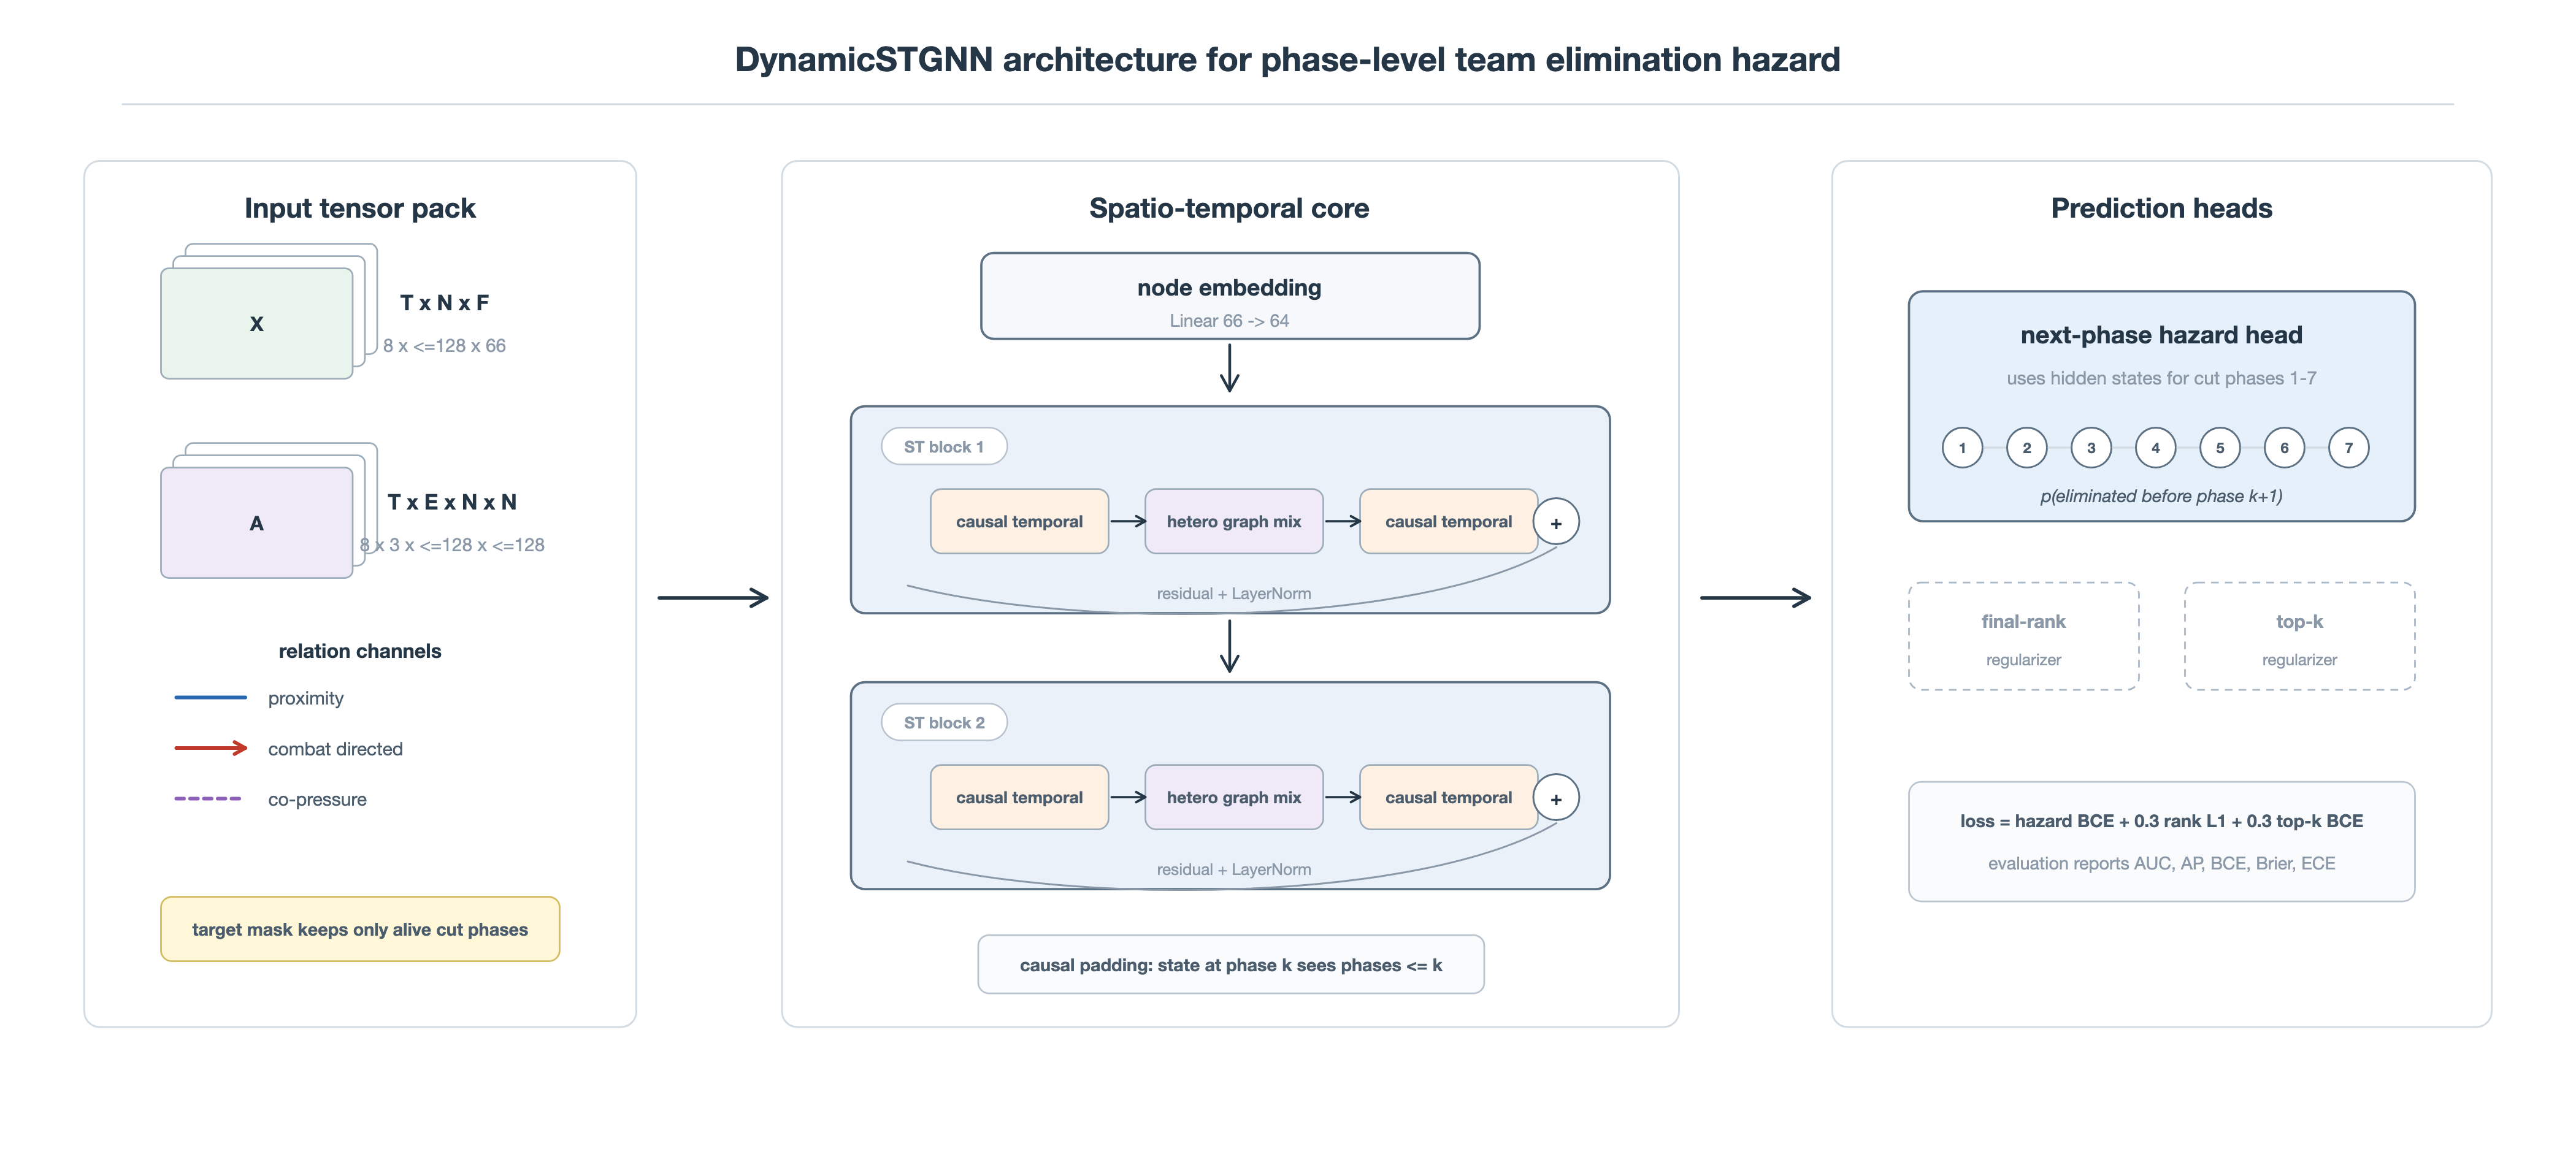
\includegraphics[width=0.86\textwidth]{figures/dynstgnn_architecture.png}
\caption{DynamicSTGNN. (a) 입력은 phase당 하나의 heterogeneous team
graph이며 proximity, combat, co-pressure 세 relation channel을 갖는다. (b)
Network는 node feature를 embedding한 뒤 gated spatio-temporal block 두 개를
쌓고 hazard head로 출력한다. (c) 각 ST block은 gated causal temporal convolution, relation channel별로 집계해
학습된 softmax weight와 skip connection으로 결합하는 heterogeneous graph
convolution, 두 번째 gated temporal convolution, 그리고 residual connection을
갖는 layer normalization을 적용한다. Causal padding은 phase \(k\)가 이후
phase를 보지 못하게 한다.}
\label{fig:dynstgnn-arch}
\end{figure*}

Ablation은 no edge, proximity only, proximity plus combat, full graph 네
조건을 비교한다. 또한 같은 team-phase row의 tabular view를 사용하는
histogram gradient boosting baseline과 비교한다. 두 기준 model의 역할은
구분된다. Boosting baseline은 graph model이 같은 표현 위의 강한 tabular
learner를 이기는지 검증하고, no-edge DynamicSTGNN은 관계 adjacency만 제거한
채 architecture, temporal convolution, parameter 수, multi-task
regularization을 통제한다. 두 기준 model 모두 node feature 안에 수작업
이웃 요약(주변 적 밀도, 최근접 적 거리)을 이미 받으므로, 이를 이긴다는
것은 그런 요약으로 포착되지 않는 관계 구조에 이득을 귀속시킨다. 두 기준을
모두 개선할 때에만 dynamic team relation의 signal을 주장한다. 이 결론은 두
가지 통제로 추가 검증한다. 이득이 정말 "누가 누구와 관계 맺는가"에서
온다면 추론 시 관측 graph 안에서 team identity를 섞었을 때 이득이 사라져야
하고, 학습을 서로 다른 random seed로 반복해도 이득이 유지되어야 한다.
